% chapters/cap1_introduccion/cap1.tex

\chapter{Introducción y Motivación}

\section{La dinámica de fluidos computacional y sus límites}

La dinámica de fluidos computacional (CFD) es la disciplina que permite resolver de forma numérica las ecuaciones de Navier-Stokes para describir el movimiento de fluidos \cite{Raman2018CFDReview}. Históricamente ligada a la industria aeroespacial, hoy es una herramienta transversal crítica en diversas áreas de la ciencia y la ingeniería. Sus aplicaciones abarcan desde la meteorología y el clima, para predecir la dispersión de contaminantes \cite{Pantusheva2022PollutionCFD}; pasando por la aerodinámica en la industria automotriz y aeroespacial para la optimización de perfiles alares \cite{Slotnick2014CFDV2030}; hasta llegar a la biomedicina, donde simula complejas interacciones en la hemodinámica de arterias y ventrículos \cite{Toma2017SPHBiomedical}. 

A pesar de su éxito, la CFD clásica se enfrenta a un severo cuello de botella. Tanto los métodos basados en malla como los enfoques sin malla como \emph{Smoothed Particle Hydrodynamics} (SPH) exigen recursos masivos para evaluar las interacciones físicas a medida que aumenta la resolución. Aunque herramientas como SPH son excelentes para manejar grandes deformaciones sin necesidad de remallar, la carga combinatoria de buscar partículas vecinas en cada iteración sigue planteando tiempos de ejecución muy restrictivos a nivel industrial. Este TFM no resuelve ese cuello de botella, se busca estudiar el caso mínimo de dos partículas SPH fijas.

Para ilustrar la versatilidad de estas simulaciones, la figura \ref{fig:particles_combined} muestra la aplicabilidad del método de mallas y de la formulación SPH.

\begin{figure}[htbp]
    \centering
    % Primera subfigura (Cráneo)
    \begin{subfigure}[b]{0.48\textwidth}
        \centering
        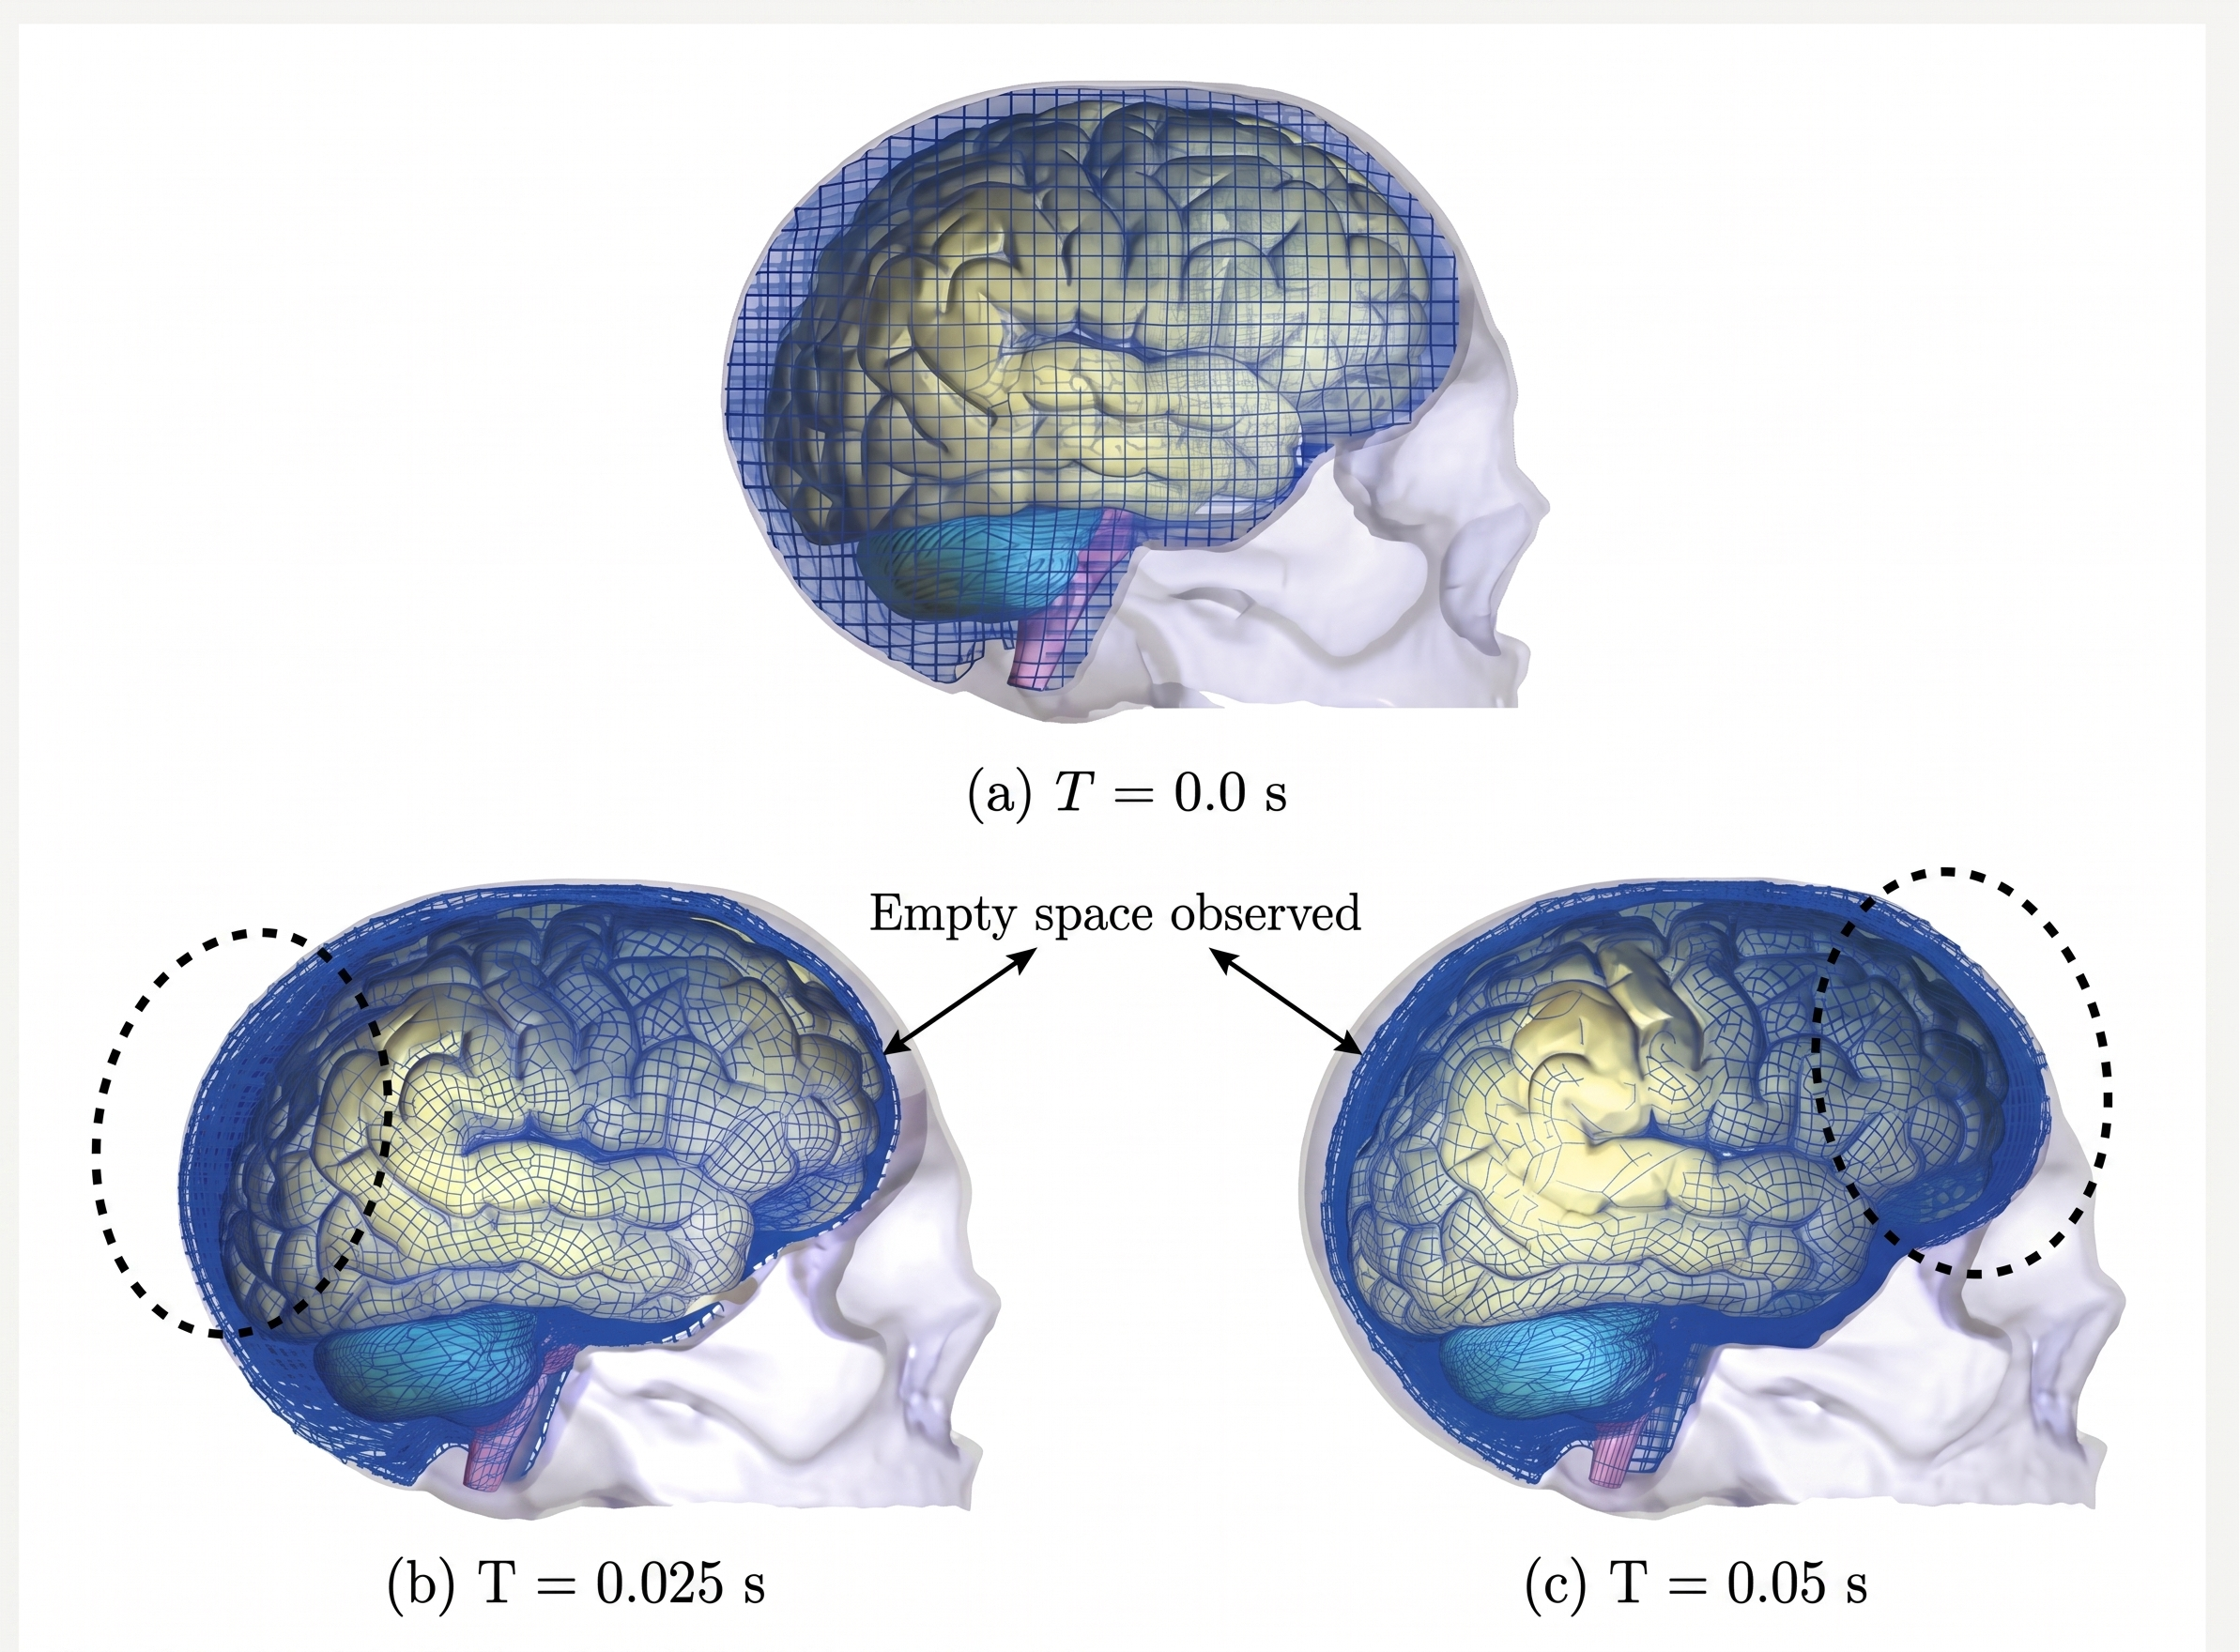
\includegraphics[width=\textwidth]{chapters/cap1_introduccion/img/craneo.png}
        \caption{Simulación de aceleración y desaceleración, mostrando la hemodinámica dentro del cráneo. Adaptado de \cite{Toma2017SPHBiomedical}.}
        \label{fig:craneo_sph}
    \end{subfigure}
    \hfill
    % Segunda subfigura (Parque eólico)
    \begin{subfigure}[b]{0.48\textwidth}
        \centering
        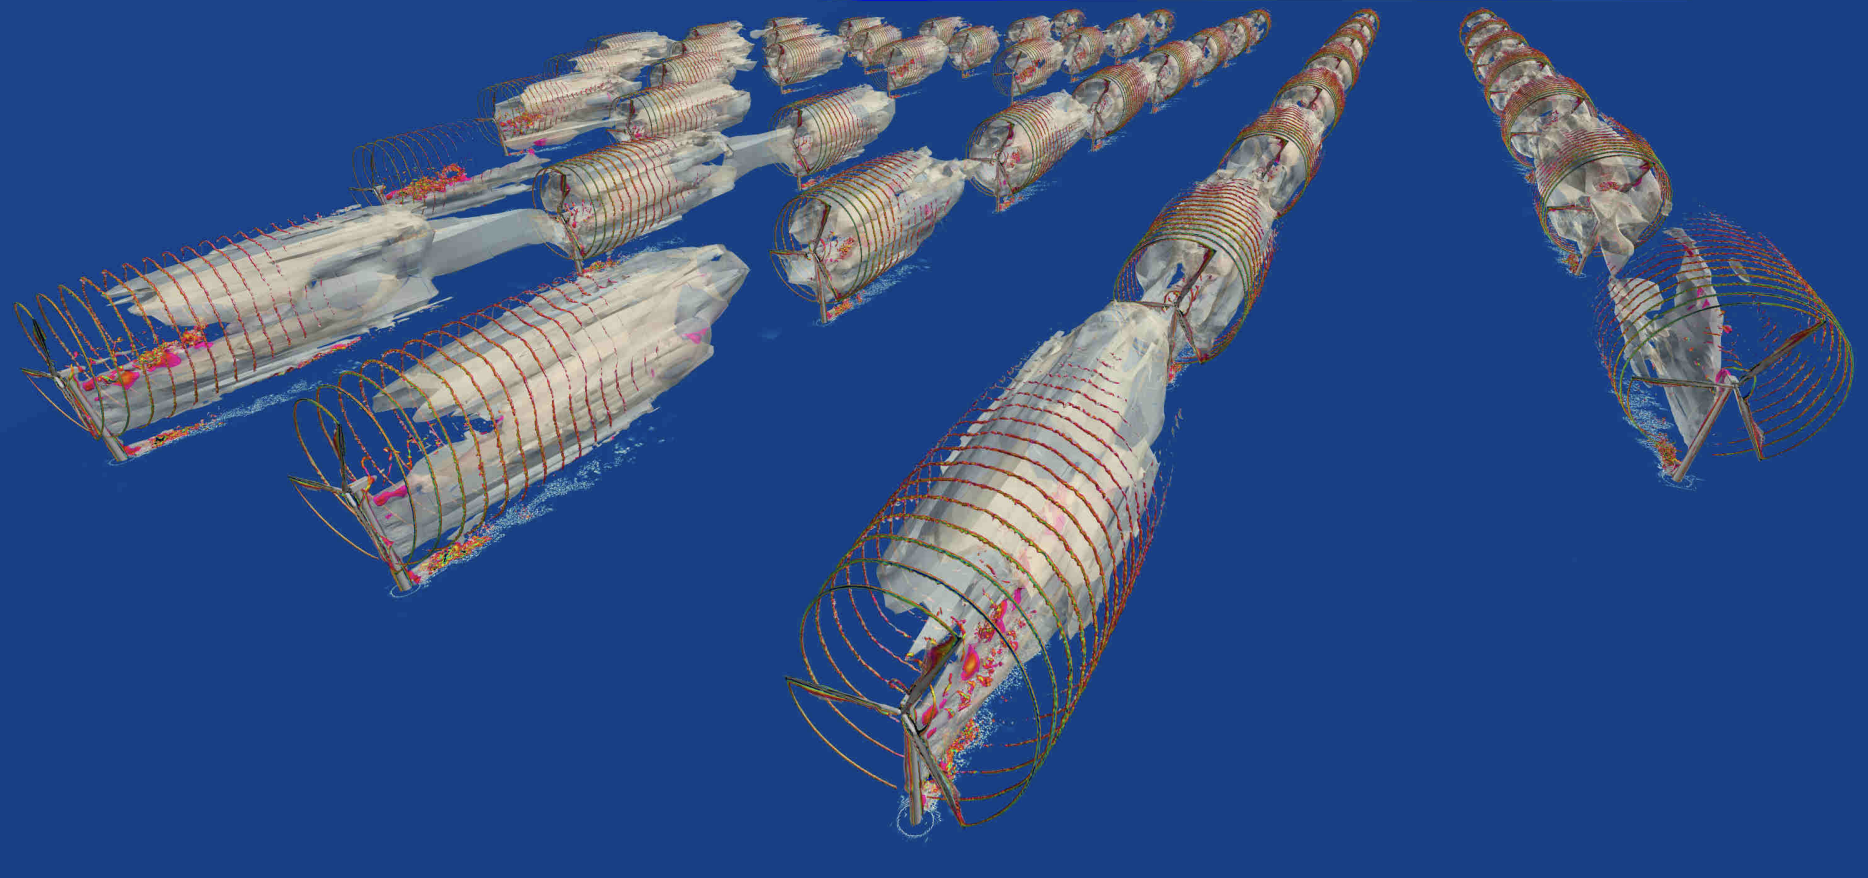
\includegraphics[width=\textwidth]{chapters/cap1_introduccion/img/turbine.png}
        \caption{Estructuras de estela en el parque eólico Lillgrund. Adaptado de \cite{Kirby2018}.}
        \label{fig:windfarm_wake}
    \end{subfigure}
    
    \caption{Ejemplos de simulación en dinámica de fluidos. (a) Hemodinámica craneal, adaptado de Toma (2017). (b) Estelas en el parque eólico Lillgrund, adaptado de Kirby et al. (2018).}
    \label{fig:particles_combined}
\end{figure}

\section{Paso de computación clásica a un modelo cuántico}

La computación cuántica surge como una vía prometedora para superar estas barreras algorítmicas clásicas. Más allá del rigor matemático, este proyecto nace de una intuición abstracta sobre la naturaleza del transporte. En el método de partículas (SPH), el fluido se discretiza en nodos que interactúan según un kernel de suavizado. Si representamos esta estructura como un grafo de interacciones, el flujo del fluido puede interpretarse como el recorrido de información a través de dicho grafo. Existe una analogía profunda entre cómo un fluido físico se desplaza y cómo la amplitud de probabilidad cuántica explora un espacio de estados en un grafo.

Investigaciones recientes han propuesto algoritmos de \emph{Quantum Smoothed Particle Hydrodynamics} (QSPH) para mapear la ecuación de advección clásica a circuitos cuánticos, destacando los notables trabajos de Au-Yeung, Williams et al. \cite{auyeung2024, auyeung2025}. Si bien el presente documento se fundamenta en gran medida en su exhaustivo estudio basado en Caminatas Cuánticas en Tiempo Discreto (DTQW), dicho enfoque presenta ciertas limitaciones, como la necesidad de registros auxiliares de moneda (\emph{coin register}) y la aparición de algunos términos adicionales en el cálculo. Por ello, nuestra metodología de implementación busca explorar un camino diferente para evaluar si es posible alcanzar una solución más directa o eficiente para el mismo problema físico.

\section{Justificación del proyecto}

La motivación principal de este proyecto es buscar una alternativa para determinar un primer paso hacía otro camino en busca de alguna mejora con respecto al estado del arte actual en QSPH, implementando Caminatas Cuánticas en Tiempo Continuo (CTQW). En este paradigma, el hamiltoniano del sistema puede construirse directamente a partir de la matriz de adyacencia de los coeficientes del kernel SPH, lo que podría simplificar la formulación de la evolución del fluido sin requerir registros adicionales.

El interés en explorar esta alternativa radica en un problema crítico de la industria, debido a que la dinámica de fluidos computacional (CFD) de alta fidelidad representa una de las mayores cargas de trabajo en los superordenadores modernos a nivel global \cite{Karp2024CFDMSA}. Por ejemplo, simulaciones recientes de dinámica de fluidos en el superordenador de exaescala \textit{Frontier} (Oak Ridge National Laboratory, EE. UU.) han requerido paralelizar billones de puntos de malla y miles de GPUs durante horas para resolver problemas aeroespaciales y energéticos, acaparando una inmensa fracción del consumo energético y de los ciclos de CPU/GPU de estas instalaciones \cite{OakRidge2025FrontierCFD}.

Dada la altísima relevancia de aplicaciones como el diseño aeroespacial, la optimización automotriz y la biomedicina, acelerar estas dinámicas es una necesidad tecnológica urgente. Por tanto, este trabajo investiga si un CTQW, compilado con \emph{Matching Decomposition}, puede reproducir la discretización SPH \eqref{eq:sph_advection_discrete} en el dímero de dos partículas fijas. \emph{Matching Decomposition} se adopta como método de compilación \cite{matching2026}; en $N=2$ no se demuestra reducción de profundidad ni alivio de la demanda CFD en hardware NISQ. El criterio de éxito es la correspondencia cualitativa con la ecuación \eqref{eq:sph_advection_discrete}, no una aceleración industrial.
